%!TEX root = ../../thesis.tex


\section{Keplerian Orbits}

When two bodies are in orbit (two stars or a star and a planet) they orbit about their common centre of mass. Their 3-dimensional motion can be derived with a combination of Newton's universal law of gravitation, and Kepler's laws.
The full derivation is quite long and can be commonly found in several celestial mechanics texts~\citep[e.g.][]{moulton_introduction_1914, perryman_exoplanet_2011}. The notes given here mainly follow \citep{valiero__2016}. 

\begin{figure}
    \centering
    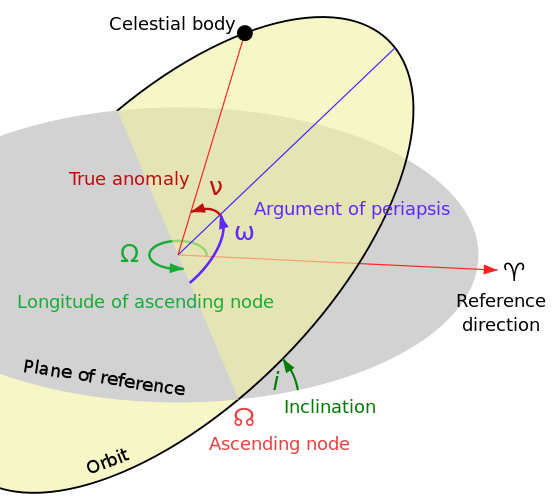
\includegraphics[width=0.3\linewidth]{figures/advanced_material/orbit}
    \caption{The basic elements of the Keplerian orbit. Credit \href{https://commons.wikimedia.org/w/index.php?curid=8971052}{Lasunncty}.}
    \label{fig:orbit}
\end{figure}
\todo{The plot from summer school book would be better}

\Cref{fig:orbit} shows the basic elements of the Keplerian orbit. There are several parameters required to situate the orbit in space. There is a \textit{reference plane}, tangential to the celestial sphere, that cuts the orbital plane with a \textbf{line of nodes}. The \textbf{ascending node} is the point on the plane at which the body crosses the reference plane moving away from the observer, and is defined relative to the vernal reference point, \Aries, with the \textit{longitude of the ascending node}, $\Omega$, setting the orientation. 

To fully parametrize a Keplerian orbit requires seven parameters. These are: $a$ the semi-major axis of the elliptical orbit, $e$ the orbital eccentricity, $P$ orbital period, $T_0$ the \emph{time of periastron passage}, $i$ orbital inclination relative to the line of sight, $\omega$ the \emph{argument of periastron}, and $\Omega$.
From RV measurements alone all of these parameters except for $i$ and $\Omega$ can be determined. $\Omega$ is irrelevant for determining the orbital mass, but inclination $i$ is very important as it effects the projection of the velocity towards the observer.

With system of two bodies with masses $\mone$ and $\mtwo$, under the force of gravity their orbits describe elliptical orbits as seen in \cref{Figure}. In polar coordinates the ellipse of an orbit for each a body with the centre of mass at one focus is described by:
\begin{equation}
    r = \frac{a(1-e^{2})}{1 + e \cos(\nu(t))},
\end{equation}
where $a$ is the length of the semi-major axis for the body, $e$ is the eccentricity, $\nu$ is the \emph{true anomaly} the angle between the current position of the orbiting body and periastron.

The true anomaly is not only a function time, \(t\), but also the orbital period \(P\), the \emph{time of periastron passage}, \(T_0\), and eccentricity. It is geometrically related to the eccentric anomaly:
\begin{equation}
\cos(\nu(t)) = \frac{\cos(E(t))}{1 - e \cos(E(t))}
\end{equation} 
which can be numerically determined from the mean anomaly M(t):
\begin{equation}
M(t) = \frac{2 \pi}{P}(t - T_0) = E(t) - e \sin(E(t))
\end{equation}
The mean anomaly is the angle for the average orbital motion of the body at a time after periastron passage \(t-T_0\).

\missingfigure{elipical orbit plot}

From Kepler's second law\footnote{Orbit sweeps out equal areas in equal times} \(1/2 r^{2} d\nu/dt\) = constant, while in one full period P, the total area of the ellipse \(\pi a^{2}{(1 - e^{2})}^{1/2} \) will be covered, leading to: 
\begin{equation}
r^2 \frac{d\nu}{dt} = \frac{2\pi a^{2}(1-e^{2})^{1/2}}{P} \label{eqn:kepler_area}
\end{equation}

The radial velocity is the change in $r$ along the line of sight $z$. The component of $r$ along the line of sight (from \cref{fig:orbit}) is:
\begin{equation}
   r_z =  r_1 \sin(\nu_1(t) + \omega)\sin(i) + \gamma \label{eqn:r_z}
\end{equation}
where $\gamma$ is the mean velocity of the barycentre, and the subscripts `1' and `2' refer to the star and planet (or companion star), respectively.
Differentiating \cref{eqn:r_z} and substituting in \cref{eqn:kepler_area} leaves the common RV equation:
\begin{equation}
\label{eqn:rv_equation}
{RV} = \dot{r}_z= \frac{2 \pi a_1 \sin(i)}{P{(1-e^{2})}^{1/2}} [\cos{(\nu(t) + \omega)} + e\cos{(\omega)}] + \gamma
     = K_1 [\cos{(\nu(t) + \omega)} + e\cos{(\omega)}] + \gamma,
\end{equation}
where several parameters and constants have been condensed into $K$, referred to as the \emph{semi amplitude}. In this case $\kone$ is the semi amplitude for the star.


\subsection{Mass function}

Once the orbital parameters have been determined then it is possible to determine the mass function of the system. From the centre of mass the distance between the two bodies is \(a = a_1 + a_2\) where $a_1$ and $a_2$ are the respective distances to the barycentre, while the value \(\mone a_1 = \mtwo a_2\) can allow these rearrangements:
\begin{equation}
a = a_{1} (1 + \frac{a_{2}}{a_{1}}) = a_{1}(1 + \frac{M_{1}}{M_{2}}) = \frac{a_{1}}{M_{2}} (M_{1} + M_{2})
\end{equation}

Kepler's third law can be written as:
\begin{equation}
    \frac{G}{4\pi^{2}}(M_{1} + M_{2})P^{2} = {(a_1 + a_2)}^{3}
\end{equation}

\begin{equation}
\frac{G}{4\pi^{2}}(M_{1} + M_{2})P^{2} = a_{1}^{3}{(\frac{M_{1} + M_{2}}{M_{2}})}^{3}
\end{equation}
replacing $a_1$ with $K_1$ from \cref{eqn:rv_equation} results in the mass function $f(M)$:
\begin{equation}
f{M} = \frac{{(M_{2}\sin(i))}^{3}}{{(M_{1} + M_{2})}^{2}} = K^3_1 P {(1-e^{2})}^{3/2}
\end{equation}

This function can be determined directly from the measurable parameters $P$ $e$ and $K_1$. It also depends on the stellar mass $M_1$, which needs to be known  (by some other means) to determined the planet mass. Also from this function that the true mass of the planet $M_2$ is not obtained but only the projected mass $M_{2}\sin{i}$.

For a planetary companion the approximation $M_2 \ll M_1$ can be made and for circular orbit the radial velocity semi-amplitude can be re-written as:

\begin{equation}
K_1 = \frac{28.4}{\sqrt{1-e^{2}}} \frac{\mtwosini}{\Mjup} {\left(\frac{\mone}{\Msun}\right)}^{-2/3} {\left(\frac{P}{1 yr}\right)}^{-1/3}  [\mps]
\end{equation}

This can be used to calculate the RV amplitude create by different mass planets in various circular orbits as given in \cref{}.

\todo{Find the table to velocities}


\subsection{{RV} calculation}
\unfinished{Move location / adjust from paper}
We use the Keplerian orbit {RV} equation (\cref{eqn:rv_equation}) to estimate the {RV} of the host and companions at the time of each observation, \(t\):

The literature parameters for each target are provided in \cref{tab:orbitparams}.


To determine the {RV} of the companion we transformed the {RV} semi-amplitude of the host \(\kone\) into the semi-amplitude for the companion \(\ktwo\) using the mass ratio,
\begin{equation}
\label{eqn:mass_ratio}
q = \mtwo / \mone = \kone / \ktwo
\end{equation}

We note that for the targets in which only the minimum mass (\mtwosini) is known, this equation will indicate the maximum \(\ktwo\) value for the companion.
The estimated \(\ktwo\) for each companion is provided in \cref{tab:estimatedparameters} while the {RV} for both components at the time of each observation is provided in \cref{tab:observations}.


\todo{Possibly just move this too the place where it is used.}
The error on estimated {RV} values, shown in \cref{fig:HD211847_result_contours}, is calculated by applying the general error propagation formula~\citep{ku_notes_1966} and using the errors on the orbital parameters.
For a function, \(f\), with errors on the inputs \(\delta x\), \(\delta y\) etc., it follows:
\begin{align}
f &= f(x, y, z, \ldots)\\
\delta f &= \sqrt{{\left( \frac{\partial f}{\partial x} \delta x\right)}^2 + {\left(\frac{\partial f}{\partial y} \delta y\right)}^2 + {\left(\frac{\partial f}{\partial z} \delta z\right)}^2 + \ldots}.
\end{align}




% from draft of paper 18/7/2017
\subsection{Companion K}  Maybe something can go above from this...
\label{sec:companion_RV}
\emph{These sections might be unnecessary}\\

To calculate the {RV} of the companion at the time of each observation.
For a two-body system the {RV} semi-amplitude of the companion \(\ktwo\) can be determined from the orbital host-companion mass ratio
\begin{equation}
q = \mone/\mtwo = \ktwo/\kone\label{eqn:q_ratio_K2}.
\end{equation}
Note, that for the targets in which only the minimum mass (\mtwosini) is known, this will give the maximum {RV} semi-amplitude of the companion.
This relation was used to estimate \(\ktwo\) for the companion from the minimum mass or mass we have for each companion.
These values along with the other orbital parameters of the system were used to calculate the {RV} of the companions for each observation.
These values are provided with the observations in \cref{tab:observations}.




If more than one planet is present then they gravitationally influence each other and their orbits become non-Keplerian, i.e.\ a N-body problem? {\textbf{ref}}.
In this work were a star has two companions we will only assume Keplerian orbits for the companion, independently.
